\begin{figure}[!ht]
    \begin{center}
      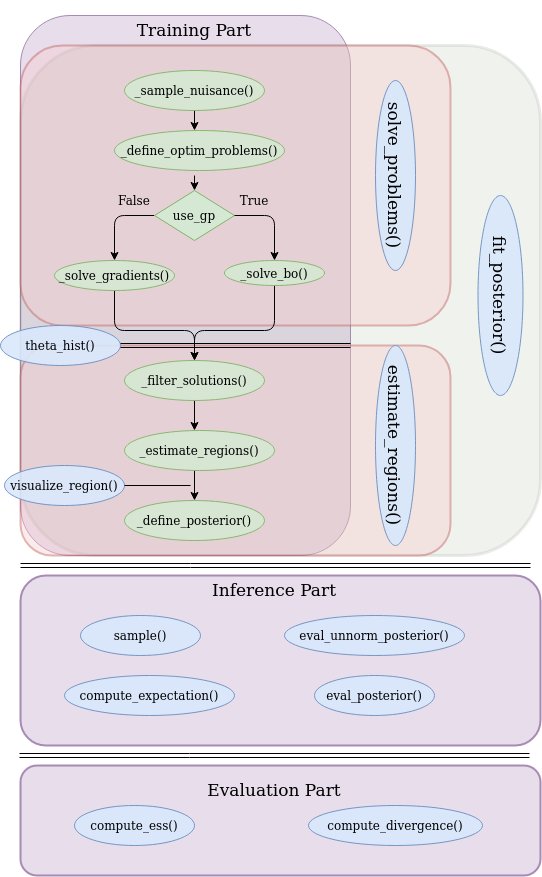
\includegraphics[width=0.75\textwidth]{./Thesis/graphs/ROMC.png}
    \end{center}
    \caption{Overview of the ROMC implementation. The training part follows a sequential pattern; the functions in the green ellipses must be called in a sequential fashion for completing the training part and define the posterior distribution. The functions in blue ellipses are the API calls that are called by the user.}
    \label{fig:elfi-model}
\end{figure}